\section{RESULTS AND DISCUSSION}

This chapter presents the experimental results obtained from the four neural network architectures described in Section~\ref{subsec:models}, evaluated first on the held-out synthetic test partition (Subsection~\ref{subsec:synth_results}) and then on a real-world dataset acquired from a human piloted UAV in a coastal site (Subsection~\ref{subsec:real_results}). Subsection~\ref{subsec:model_comparison} provides a comparative analysis of the architectures in terms of size, complexity, and practical deployment considerations.

\subsection{Synthetic Test Set Evaluation}
\label{subsec:synth_results}

The synthetic test partition (2{,}630 samples, stratified across 21 altitude levels from 50 to 800~cm) was used to evaluate each model's ability to regress altitude from Value-channel images drawn from the same domain as the training data. This evaluation isolates the model's learning capacity from domain-shift effects, providing an upper bound on expected accuracy before real-world deployment.

Fig.~\ref{fig:training_curves} shows the training and validation curves (Huber loss and RMSE) for all four architectures. The ResNet50-based models (top two rows) required more epochs to converge than the WaterNet variants (bottom two rows), consistent with the larger number of parameters in the regression head being optimized against a frozen backbone. The ResNet50 baseline (top row) exhibits a persistent gap between training and validation loss, indicating mild overfitting to the synthetic training distribution. In contrast, the ResNet50-Fusion model (second row) achieves tighter convergence between the two curves, suggesting that the handcrafted feature branch acts as a regularizer by providing complementary altitude-correlated signals that reduce the model's reliance on potentially spurious visual patterns.

The WaterNet baseline (third row) converges rapidly within approximately 10 epochs and reaches the lowest final validation loss among all models, despite having significantly fewer parameters than the ResNet50 variants. The WaterNet-FusionLite model (bottom row) shows similarly fast convergence with slightly higher validation loss, reflecting the trade-off introduced by the lighter convolutional backbone (three blocks instead of four, with $3\times3$ kernels instead of $5\times5$).

\subsubsection{Per-Model Prediction Analysis}

To examine prediction behavior in detail, Figs.~\ref{fig:resnet50_testplot}--\ref{fig:waternet_testplot} display the predicted altitude against the ground truth for every sample in the synthetic test set, sorted by ascending true altitude. These plots reveal how each model tracks the staircase pattern formed by the 21 discrete altitude levels.

\paragraph{WaterNet (Fig.~\ref{fig:waternet_testplot}).} The custom CNN achieves the tightest tracking of the ground-truth staircase among all models. Predictions cluster closely around the true altitude at all levels, with notably low variance in the 50--300~cm range. Beyond 400~cm, the spread increases moderately but remains smaller than that of the ResNet50 variants. The strong performance of this comparatively shallow architecture suggests that the altitude estimation task over water surfaces is well served by texture-level features captured in the early convolutional layers, and that the deeper, more abstract representations learned by ResNet50 may not provide additional benefit for this specific domain.

\begin{figure}[!h]
    \centering
    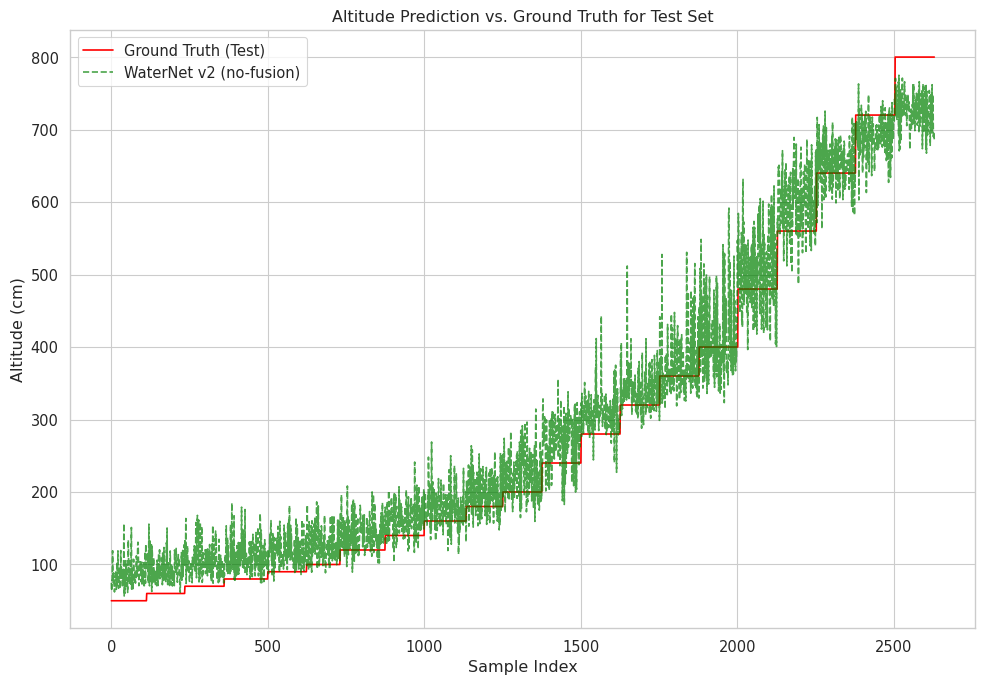
\includegraphics[width=\textwidth]{Images/WaterNet_testplot.png}
    \caption{Altitude prediction (green) vs.\ ground truth (red) for the synthetic test set using the WaterNet baseline.}
    \label{fig:waternet_testplot}
\end{figure}

\paragraph{WaterNet-FusionLite (Fig.~\ref{fig:waternet_fuslite_testplot}).} The lightweight fusion model achieves prediction quality comparable to the full WaterNet, with tight tracking at low-to-mid altitudes and slightly increased spread at the highest levels. The fact that this model uses only three convolutional blocks and $3\times3$ kernels, with roughly one-tenth the parameters of the full WaterNet, makes it a strong candidate for embedded deployment where computational resources are constrained.

\begin{figure}[!h]
    \centering
    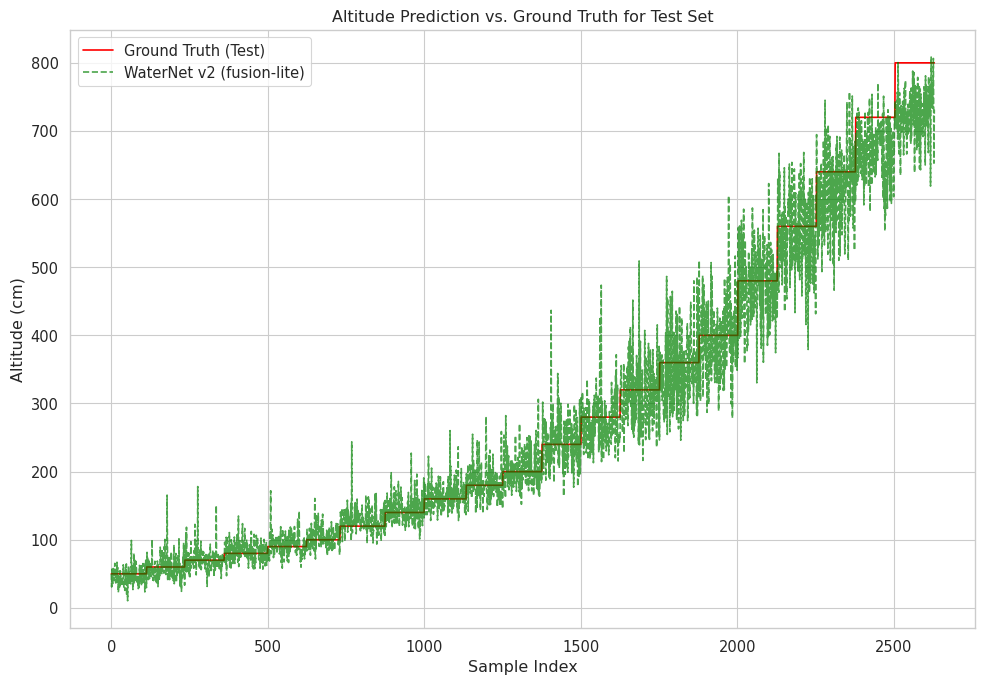
\includegraphics[width=\textwidth]{Images/WaterNet-FusLT_testplot.png}
    \caption{Altitude prediction vs.\ ground truth for the synthetic test set using the WaterNet-FusionLite model.}
    \label{fig:waternet_fuslite_testplot}
\end{figure}

\paragraph{ResNet50 (Fig.~\ref{fig:resnet50_testplot}).} The ResNet50 baseline produces high variance at nearly all altitude levels, with predictions scattering widely around the ground truth. At low altitudes (50--100~cm), predictions oscillate between approximately 50 and 200~cm, and the spread increases substantially beyond 400~cm, where individual predictions deviate by up to 300~cm from the true value. This behavior is consistent with the relatively high validation loss observed during training and suggests that the frozen ImageNet features, while powerful for natural image recognition, do not efficiently encode the fine-grained texture differences that distinguish adjacent altitude levels in water surface imagery.

\begin{figure}[!h]
    \centering
    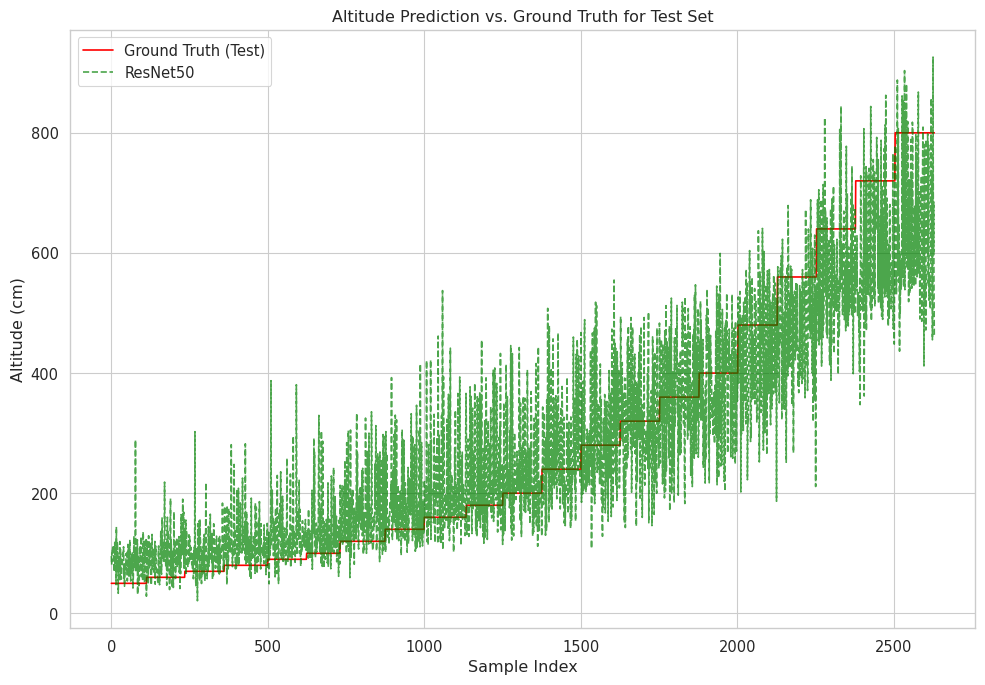
\includegraphics[width=\textwidth]{Images/ResNet50_testplot.png}
    \caption{Altitude prediction (green) vs.\ ground truth (red) for the synthetic test set using the ResNet50 baseline.}
    \label{fig:resnet50_testplot}
\end{figure}

\paragraph{ResNet50-Fusion (Fig.~\ref{fig:resnet50fus_testplot}).} The addition of the 12-element handcrafted feature vector produces a marked improvement in prediction stability. The predictions track the ground-truth staircase more closely, particularly in the 50--400~cm range, where the variance is substantially reduced compared to the ResNet50 baseline. At higher altitudes (above 500~cm), some spread remains, but the tracking of the altitude trend is preserved. This improvement indicates that the FFT energy ratios, gradient statistics, and Shi-Tomasi corner counts provide altitude-discriminative information that complements the CNN's learned representations.

\begin{figure}[!h]
    \centering
    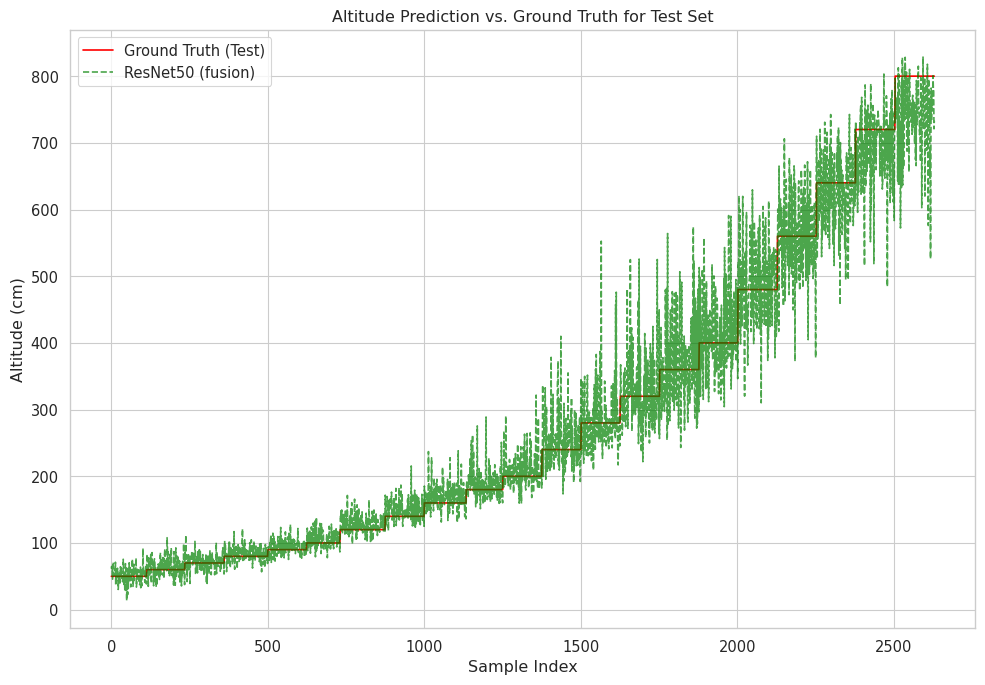
\includegraphics[width=\textwidth]{Images/ResNet50-Fus_testplot.png}
    \caption{Altitude prediction (green) vs.\ ground truth (red) for the synthetic test set using the ResNet50-Fusion model.}
    \label{fig:resnet50fus_testplot}
\end{figure}

\subsubsection{Error Distribution Analysis}

Figs.~\ref{fig:resnet50_hist}--\ref{fig:waternet_fuslite_hist} present histograms of the prediction error (predicted minus true altitude, in centimeters) for each model on the synthetic test set, overlaid with a fitted Gaussian curve to characterize the error distribution.

\paragraph{WaterNet (Fig.~\ref{fig:waternet_hist}).} The WaterNet error distribution shows a slight positive bias ($\mu = 18.7$~cm) with a standard deviation of $\sigma = 40.3$~cm. The distribution is right-skewed, with a heavier tail toward positive errors (overestimation). This systematic overestimation bias is consistent with the observation noted in the GUIDE documentation and may originate from the brightness distribution mismatch between synthetic and real samples, where synthetic images at low altitudes tend to be slightly brighter than their real-world counterparts.

\begin{figure}[!h]
    \centering
    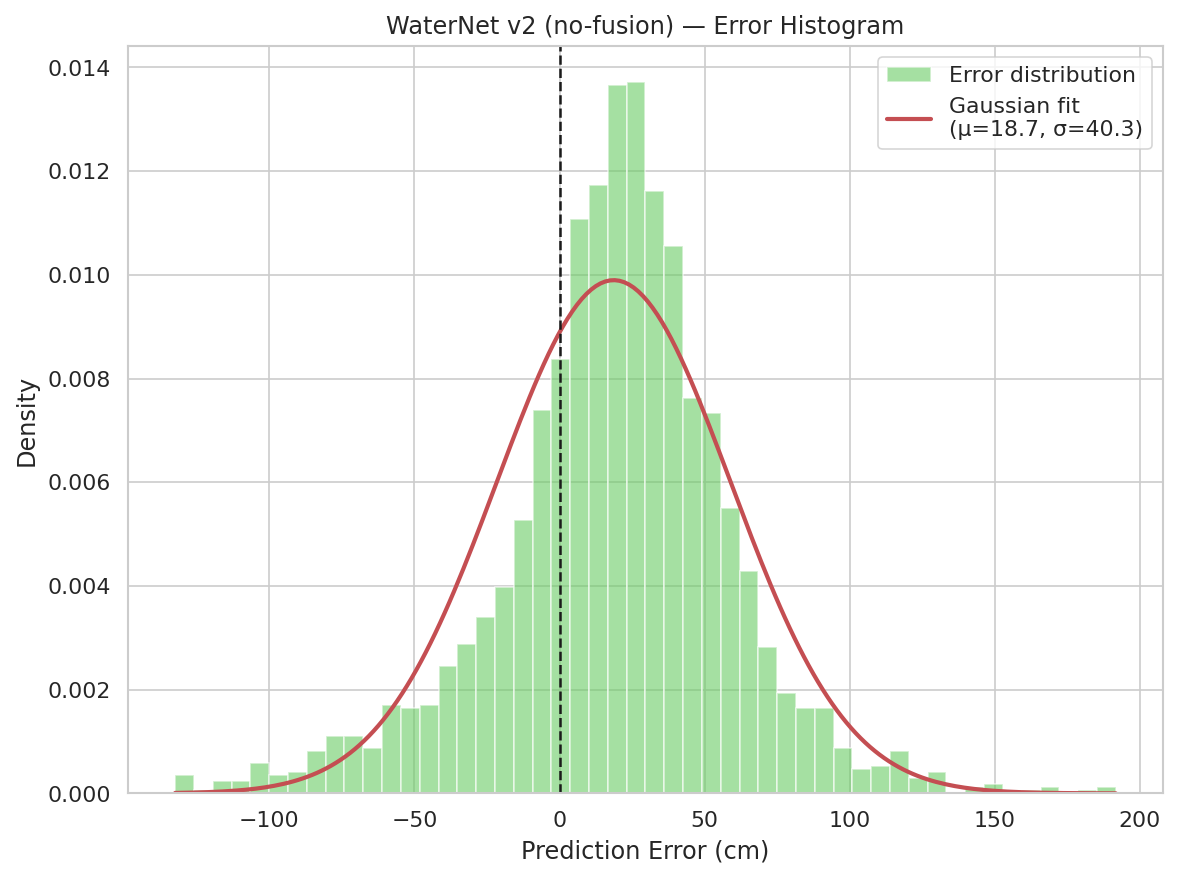
\includegraphics[width=12cm]{Images/WaterNet_histogram.png}
    \caption{Error histogram for the WaterNet baseline on the synthetic test set. The fitted Gaussian has $\mu = 18.7$~cm and $\sigma = 40.3$~cm.}
    \label{fig:waternet_hist}
\end{figure}

\paragraph{WaterNet-FusionLite (Fig.~\ref{fig:waternet_fuslite_hist}).} The lightweight fusion model achieves the most centered error distribution among the WaterNet variants ($\mu = -7.6$~cm, $\sigma = 41.7$~cm). The slight negative bias suggests a tendency toward mild underestimation. The distribution shape is approximately symmetric with moderate tails, comparable to those of the ResNet50-Fusion model.

\begin{figure}[!h]
    \centering
    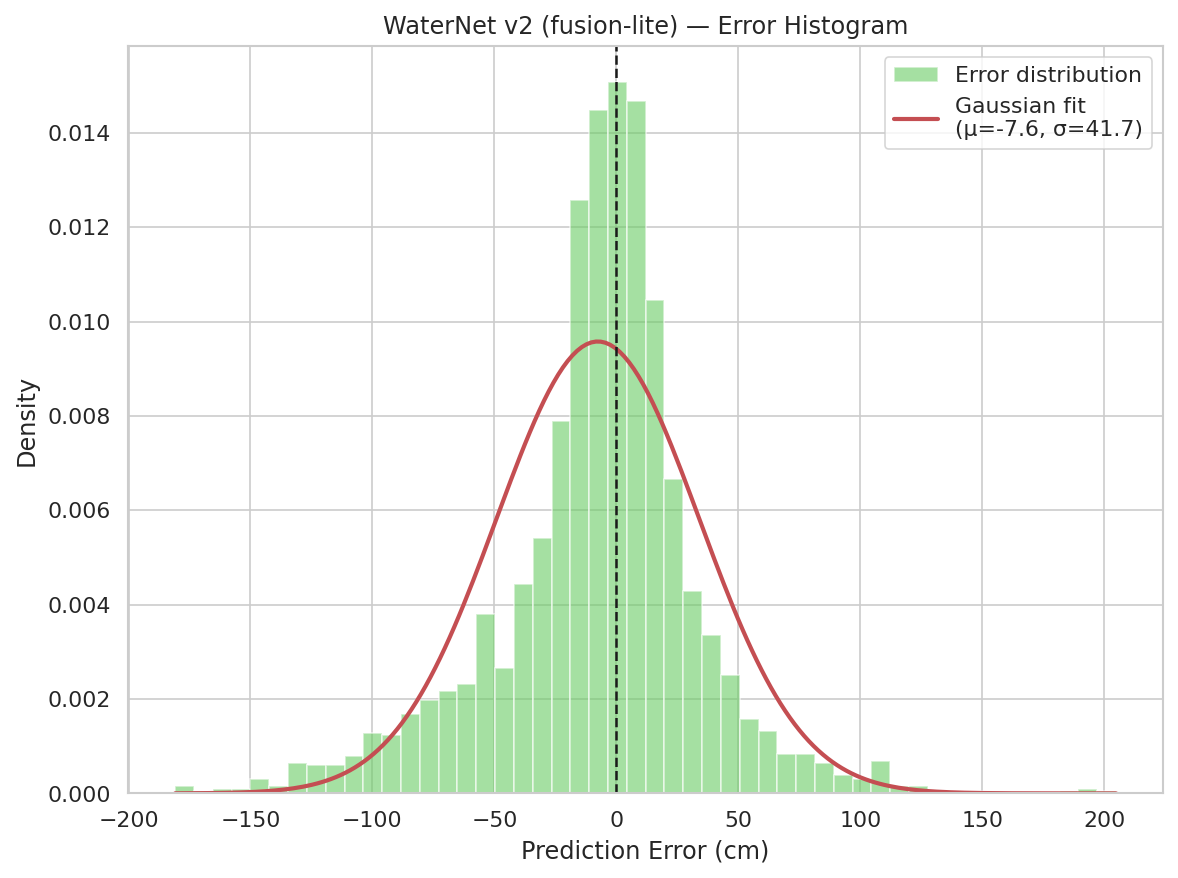
\includegraphics[width=12cm]{Images/WaterNet-FusLT_histogram.png}
    \caption{Error histogram for the WaterNet-FusionLT model on the synthetic test set. The fitted Gaussian has $\mu = -7.6$~cm and $\sigma = 41.7$~cm.}
    \label{fig:waternet_fuslite_hist}
\end{figure}

\paragraph{ResNet50 (Fig.~\ref{fig:resnet50_hist}).} The error distribution is approximately centered near zero ($\mu = -1.7$~cm) but exhibits a large standard deviation ($\sigma = 98.1$~cm), with tails extending beyond $\pm300$~cm. The Gaussian fit captures the central tendency reasonably well, although the histogram shows slightly heavier tails than a true Gaussian would predict, indicating the presence of outlier predictions.

\begin{figure}[!h]
    \centering
    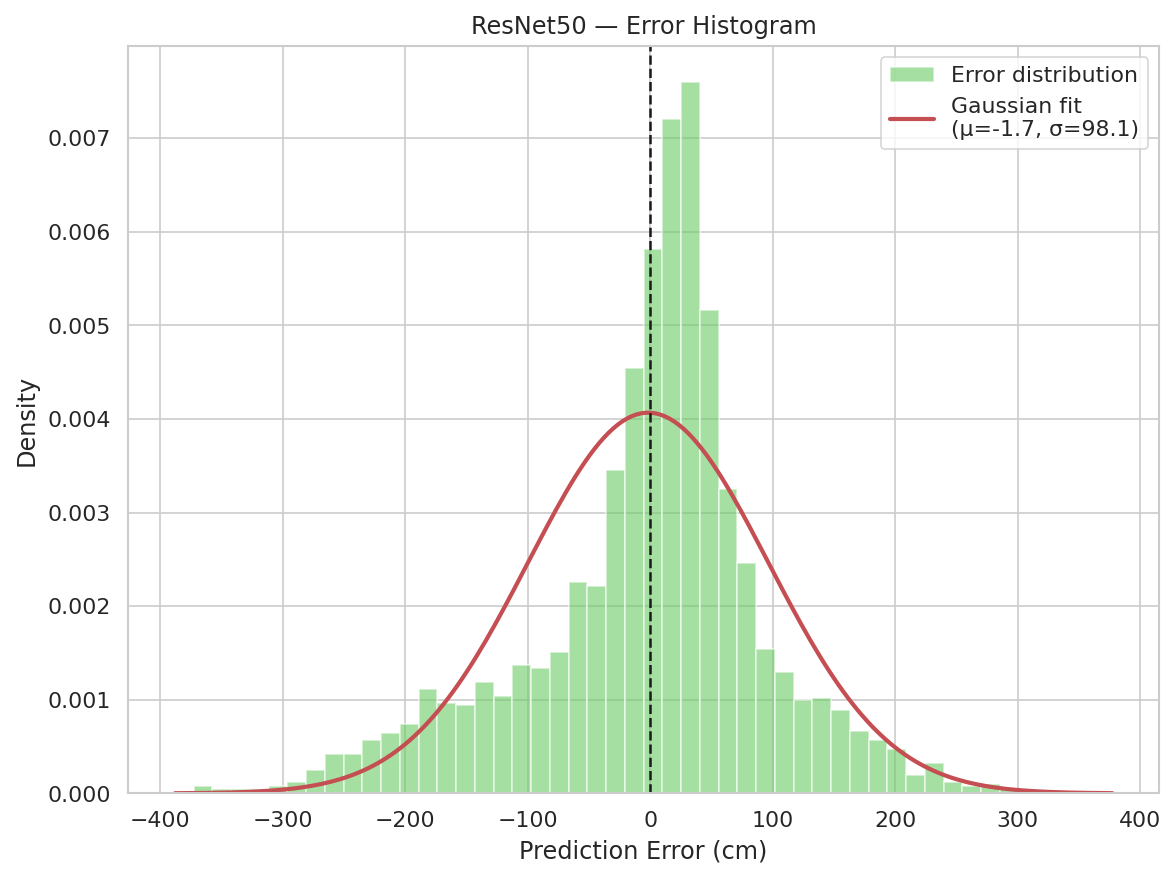
\includegraphics[width=12cm]{Images/ResNet50_histogram.png}
    \caption{Error histogram for the ResNet50 baseline on the synthetic test set. The fitted Gaussian has $\mu = -1.7$~cm and $\sigma = 98.1$~cm.}
    \label{fig:resnet50_hist}
\end{figure}

\paragraph{ResNet50-Fusion (Fig.~\ref{fig:resnet50fus_hist}).} The fusion model substantially narrows the error distribution ($\mu = 0.8$~cm, $\sigma = 44.3$~cm), reducing the standard deviation by more than half compared to the baseline. The distribution is approximately symmetric and more sharply peaked, indicating that the majority of predictions fall within $\pm50$~cm of the true altitude. The tail extent is also reduced, with errors rarely exceeding $\pm200$~cm.

\begin{figure}[!h]
    \centering
    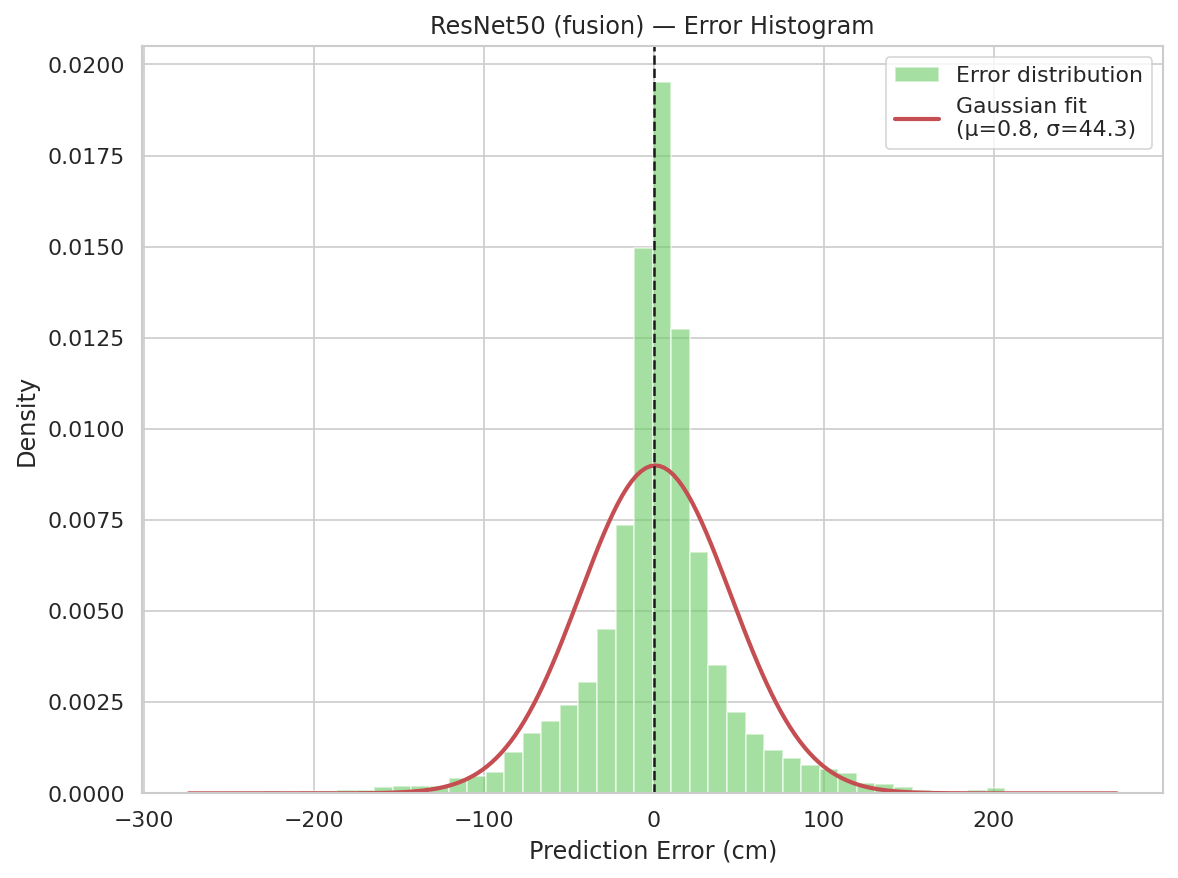
\includegraphics[width=12cm]{Images/ResNet50-Fus_histogram.png}
    \caption{Error histogram for the ResNet50-Fusion model on the synthetic test set. The fitted Gaussian has $\mu = 0.8$~cm and $\sigma = 44.3$~cm.}
    \label{fig:resnet50fus_hist}
\end{figure}

% ──────────────────────────────────────────────
\subsection{Real-World Dataset Evaluation}
\label{subsec:real_results}

The real-world evaluation dataset consists of 4{,}100 frames extracted from video captured at a coastal site, spanning an altitude range of approximately 0.8 to 12.6~m as measured by a fusion of barometric altimeter and GPS readings (the \texttt{altitude} column). A LiDAR sensor was also present during data collection and is included as a reference sensor for comparison. Importantly, none of the real images were used during training; this evaluation therefore measures the sim-to-real generalization capability of each model.

It must be noted that the ground-truth altitude measurements are themselves subject to uncertainty. The barometric-GPS fusion sensor is influenced by atmospheric pressure variations, humidity gradients, and GPS multipath effects near water surfaces. The LiDAR sensor, as discussed in Section~\ref{subsec:lidar_analysis}, proved unreliable over water due to specular reflection causing frequent zero-returns and extreme outliers (Fig.~\ref{fig:lidar_plot}). Consequently, the error metrics reported below should be interpreted as upper bounds on the true model error, since the ground truth itself carries measurement noise.

\begin{figure}[!h]
    \centering
    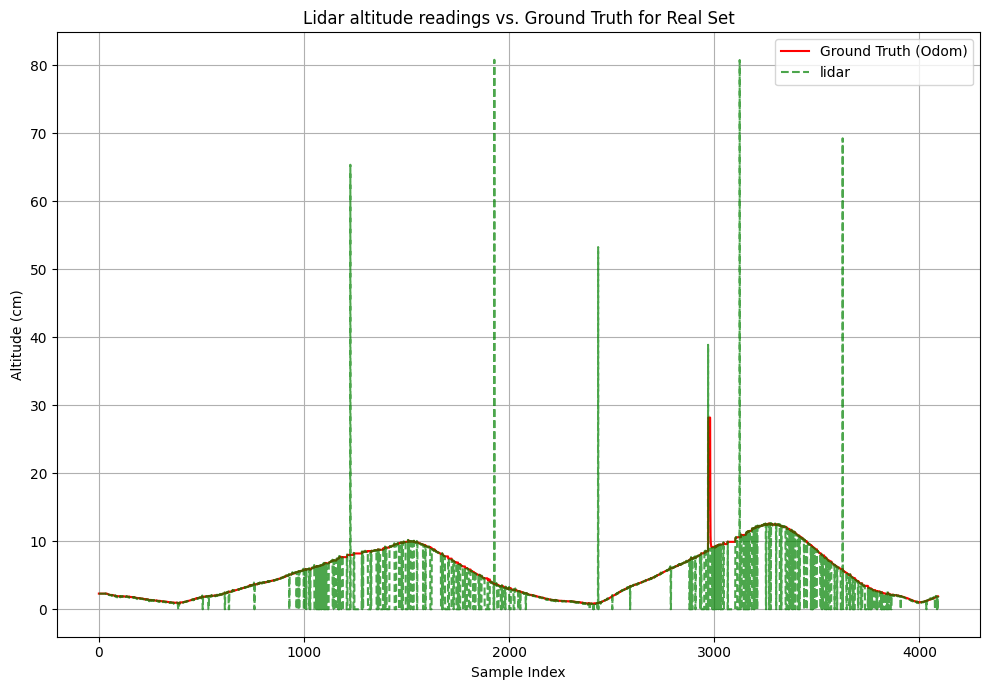
\includegraphics[width=12cm]{Images/plots/lidar_plot.png}
    \caption{LiDAR readings (green) vs ground truth (red) for the real dataset}
    \label{fig:resnet50fus_hist}
\end{figure}

The inference plot for WaterNet and WaterNet-FusLT is presented in Fig.~\ref{fig:wn_real_plot}. For ResNet50 and ResNet50-Fus, the inferences are shown in Fig.~\ref{fig:rn50_real_plot}.

\begin{figure}[!h]
    \centering
    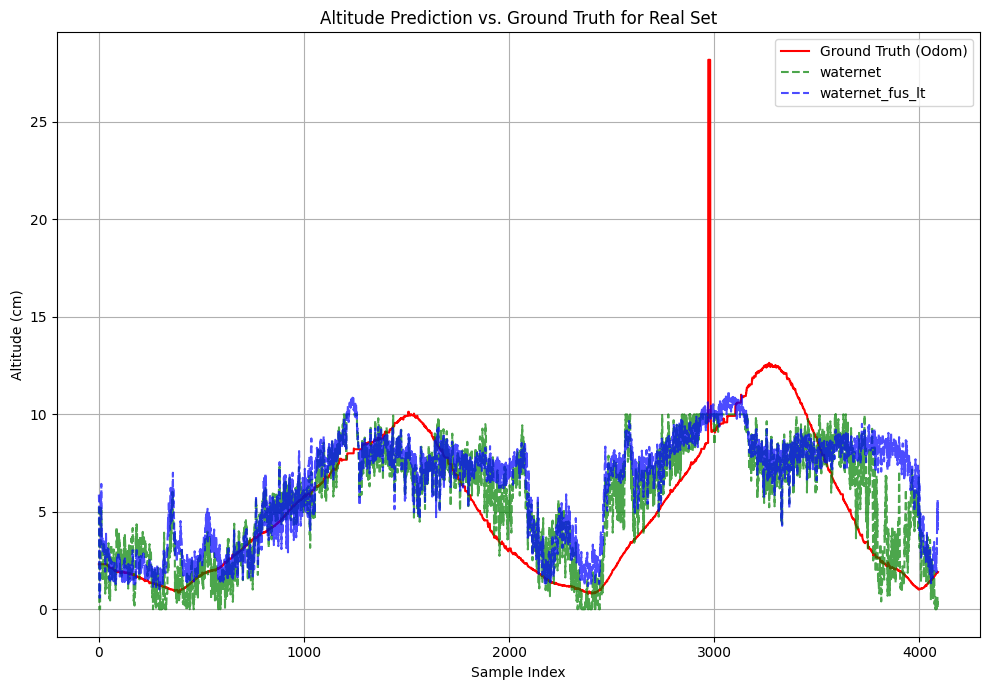
\includegraphics[width=12cm]{Images/plots/waternet_real_plot.png}
    \caption{WaterNet inference (green) vs WaterNet-FusLT inference (blue) vs ground truth (red) for the real dataset}
    \label{fig:wn_real_plot}
\end{figure}

\begin{figure}[!h]
    \centering
    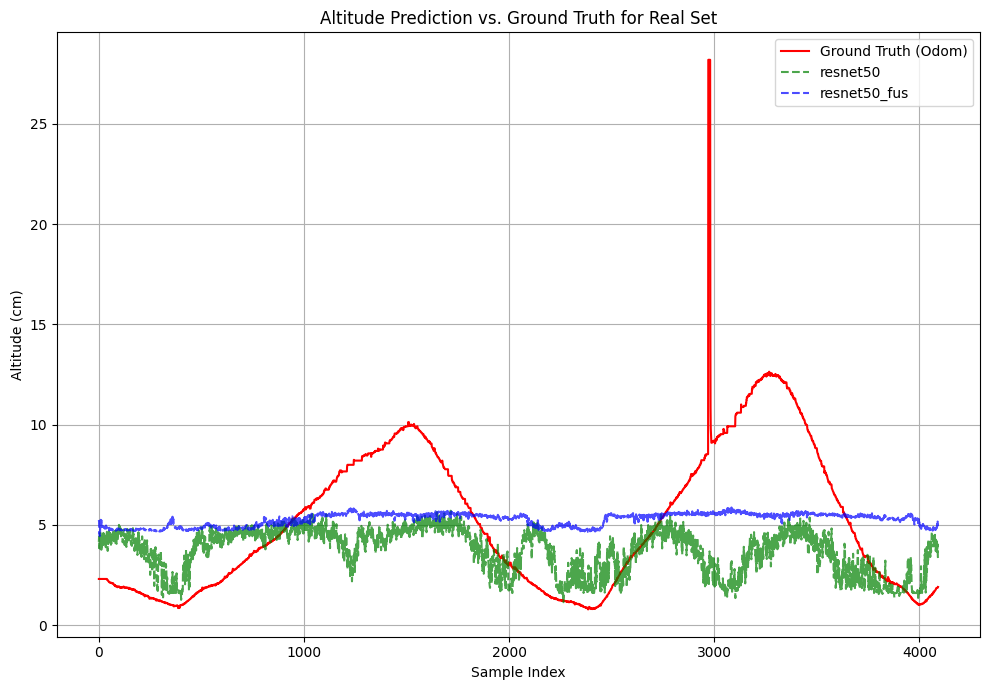
\includegraphics[width=12cm]{Images/plots/resnet50_real_plot.png}
    \caption{ResNet50 inference (green) vs ResNet50-Fus inference (blue) vs ground truth (red) for the real dataset}
    \label{fig:rn50_real_plot}
\end{figure}

\subsubsection{Aggregate Performance Metrics}

Table~\ref{tab:real_metrics} summarizes the performance of all four CNN models and the LiDAR sensor on the real-world dataset. Among the CNN models, WaterNet achieves the lowest MAE (1.787~m) and RMSE (2.337~m), with an $R^2$ of 0.551, which is the highest among all evaluated methods. The WaterNet-FusionLite model ranks second in MAE (2.208~m) and RMSE (2.859~m), followed by the ResNet50-based architectures. The ResNet50-Fusion model achieves the lowest absolute bias (0.118~m) among all CNN models, indicating that its predictions are nearly centered around the ground truth on average, despite having higher error magnitude than WaterNet.

\begin{table}[htbp]
    \caption{Performance metrics on the real-world dataset (4{,}100 frames). All error values are in meters unless otherwise indicated. Best CNN result per metric is shown in \textbf{bold}.}
    \begin{center}
        \small
        \begin{tabular}{|l|c|c|c|c|c|c|c|c|c|}
        \hline
        \textbf{Model}
            & \textbf{MAE}
            & \textbf{RMSE}
            & \textbf{Bias}
            & \textbf{$R^2$}
            & \textbf{MAPE}
            & \textbf{MedAE}
            & \textbf{P95}
            & \textbf{Max}
            & \textbf{Err.$\sigma$} \\
        \hline
        ResNet50
            & 2.700
            & 3.591
            & $-1.455$
            & $-0.061$
            & 62.82\%
            & 2.054
            & 7.985
            & 16.516
            & 3.285 \\
        \hline
        RN50-Fus
            & 2.824
            & 3.266
            & \textbf{0.118}
            & 0.122
            & 105.11\%
            & 2.939
            & 6.002
            & 12.986
            & 3.264 \\
        \hline
        WaterNet
            & \textbf{1.787}
            & \textbf{2.337}
            & 0.518
            & \textbf{0.551}
            & \textbf{57.50\%}
            & \textbf{1.373}
            & \textbf{4.875}
            & \textbf{8.680}
            & \textbf{2.277} \\
        \hline
        WN-FusLT
            & 2.208
            & 2.859
            & 1.192
            & 0.327
            & 79.54\%
            & 1.669
            & 5.760
            & 12.705
            & 2.590 \\
        \hline
        LiDAR
            & 1.697
            & 4.364
            & $-1.509$
            & $-0.567$
            & 24.78\%
            & 0.050
            & 9.700
            & 77.105
            & 4.096 \\
        \hline
        \end{tabular}
    \label{tab:real_metrics}
    \end{center}
\end{table}

Fig.~\ref{fig:benchmark_errors} presents the MAE and RMSE for all models and the LiDAR sensor side by side. The LiDAR achieves the lowest MAE (1.697~m) but the highest RMSE (4.364~m) among all methods, a diagnostic pattern indicating the presence of extreme outliers. This large gap between MAE and RMSE is characteristic of heavy-tailed error distributions: the LiDAR produces accurate readings for a subset of frames (reflected in its low median absolute error of 0.050~m) but returns severely erroneous measurements in others, inflating the squared-error penalty. In practical terms, a sensor with the lowest MAE but the highest RMSE is unreliable for safety-critical altitude control, where worst-case performance matters more than average accuracy.

\begin{figure}[!h]
    \centering
    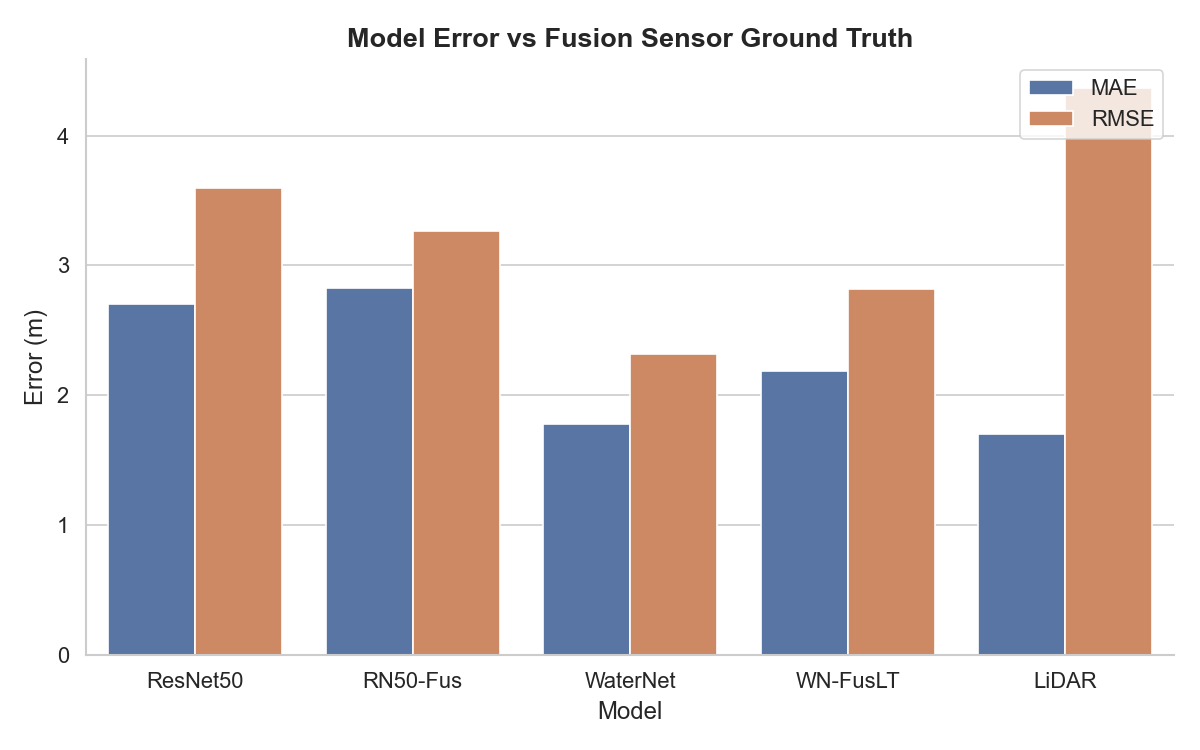
\includegraphics[width=12cm]{Images/benchmark_errors.png}
    \caption{MAE and RMSE comparison across all models and the LiDAR sensor on the real-world dataset.}
    \label{fig:benchmark_errors}
\end{figure}

\subsubsection{Systematic Bias Analysis}

Fig.~\ref{fig:benchmark_bias} shows the systematic bias (mean signed error) for each model. The ResNet50 baseline exhibits a strong negative bias ($-1.455$~m), meaning it systematically underestimates the true altitude. This underestimation is consistent with the saturation behavior observed in the scatter plot (Fig.~\ref{fig:resnet50_scatter}), where ResNet50 predictions plateau around 4--5~m regardless of the actual altitude. The LiDAR sensor shows a similar negative bias ($-1.509$~m), driven by its frequent near-zero returns over the water surface.

In contrast, the WaterNet models exhibit positive biases ($+0.518$~m for WaterNet, $+1.192$~m for WN-FusLT), indicating systematic overestimation. This upward shift is consistent with the observation from early experiments that the synthetic training domain produces images with slightly different brightness statistics than the real environment, particularly at low altitudes where synthetic images appear more greyish than their real-world counterparts.

The ResNet50-Fusion model achieves the most centered predictions, with a bias of only $+0.118$~m. This near-zero bias suggests that the handcrafted features, which are computed directly from the image statistics rather than learned from the synthetic domain, help anchor the predictions and partially compensate for the domain shift affecting the visual features.

\begin{figure}[!h]
    \centering
    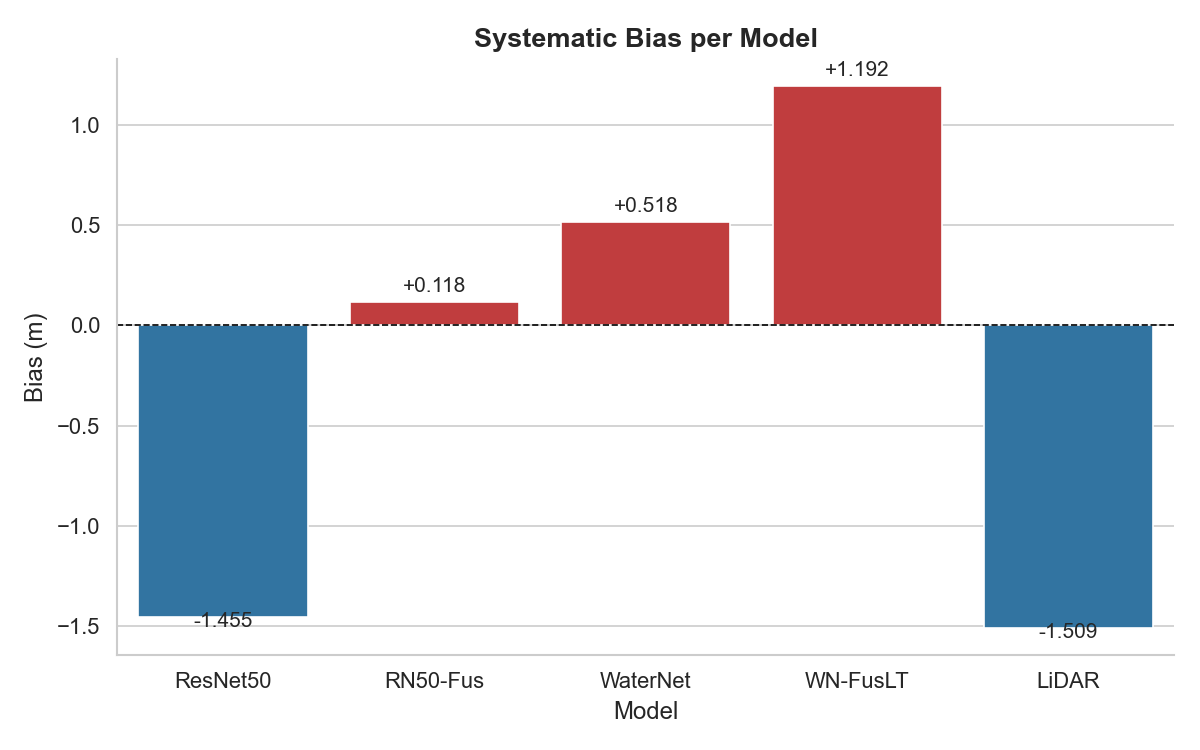
\includegraphics[width=12cm]{Images/benchmark_bias.png}
    \caption{Systematic bias (mean signed error) per model and LiDAR sensor. Positive values indicate overestimation; negative values indicate underestimation.}
    \label{fig:benchmark_bias}
\end{figure}

\subsubsection{Predicted vs.\ Ground Truth Scatter Analysis}

Figs.~\ref{fig:resnet50_scatter} and~\ref{fig:waternet_scatter} present scatter plots of predicted altitude against ground-truth altitude for the ResNet50-family and WaterNet-family models, respectively, with LiDAR included in both for reference. The dashed diagonal represents ideal ($\hat{y} = y$) predictions.

\paragraph{ResNet50 and ResNet50-Fusion (Fig.~\ref{fig:resnet50_scatter}).} The ResNet50 baseline (blue) shows a characteristic saturation pattern: predictions are compressed into a narrow horizontal band between approximately 1 and 5~m, failing to track the ground truth as altitude increases beyond 4~m. This behavior indicates that the frozen ImageNet backbone does not produce sufficiently altitude-discriminative features at the higher end of the operating range, where water surface texture differences become subtle. The ResNet50-Fusion model (orange) partially alleviates this compression, extending the predictive range upward, but still exhibits a plateau effect at higher altitudes. Both models produce a cluster of points well above the ideal line at ground-truth altitudes around 18~m, corresponding to the edge cases at the extremes of the dataset where the models extrapolate beyond their training range (50--800~cm synthetic data evaluated against real data reaching 12.6~m and beyond).

\paragraph{WaterNet and WaterNet-FusionLite (Fig.~\ref{fig:waternet_scatter}).} The WaterNet baseline (blue) tracks the ideal diagonal more closely than the ResNet50 variants across the full altitude range, though with visible positive offset (overestimation) and increasing spread at higher altitudes. The WaterNet-FusionLite model (orange) shows tighter clustering around the ideal line for altitudes below 8~m but exhibits similar dispersion at higher altitudes. Both models demonstrate that the custom-trained convolutional features, learned directly on water surface imagery rather than transferred from ImageNet, provide better domain-specific representations for this task.

The LiDAR points (green) in both plots reveal the sensor's characteristic failure mode over water: a large number of near-zero readings regardless of the true altitude, interspersed with occasional accurate measurements and rare extreme outliers (one point reaching approximately 70~m predicted for a 6~m ground truth).

\begin{figure}[!h]
    \centering
    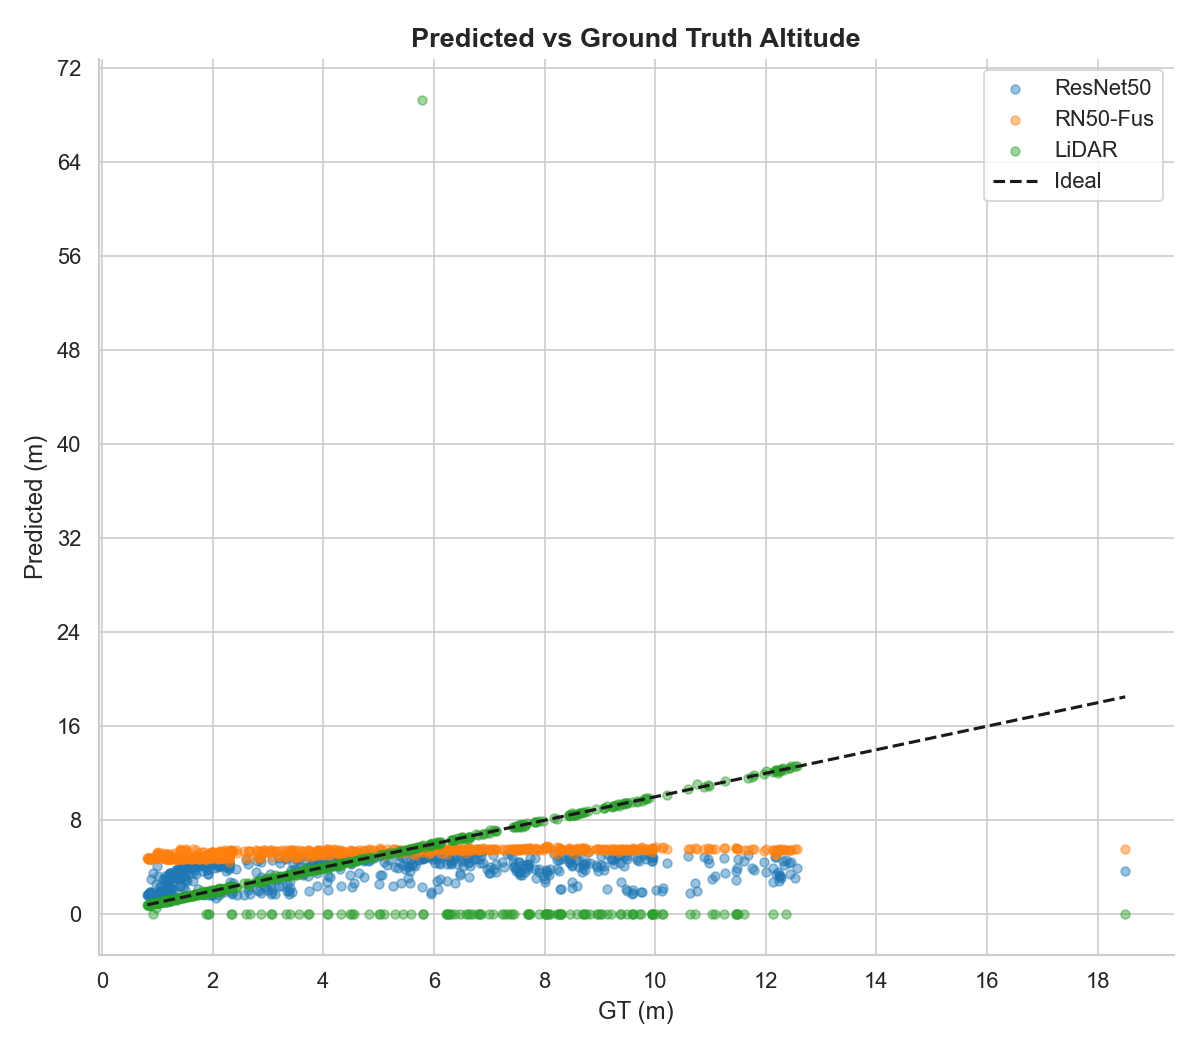
\includegraphics[width=14cm]{Images/resnet50_benchmark_scatter.png}
    \caption{Predicted vs.\ ground-truth altitude for the ResNet50 baseline, ResNet50-Fusion, and LiDAR. The dashed line represents ideal predictions.}
    \label{fig:resnet50_scatter}
\end{figure}

\begin{figure}[!h]
    \centering
    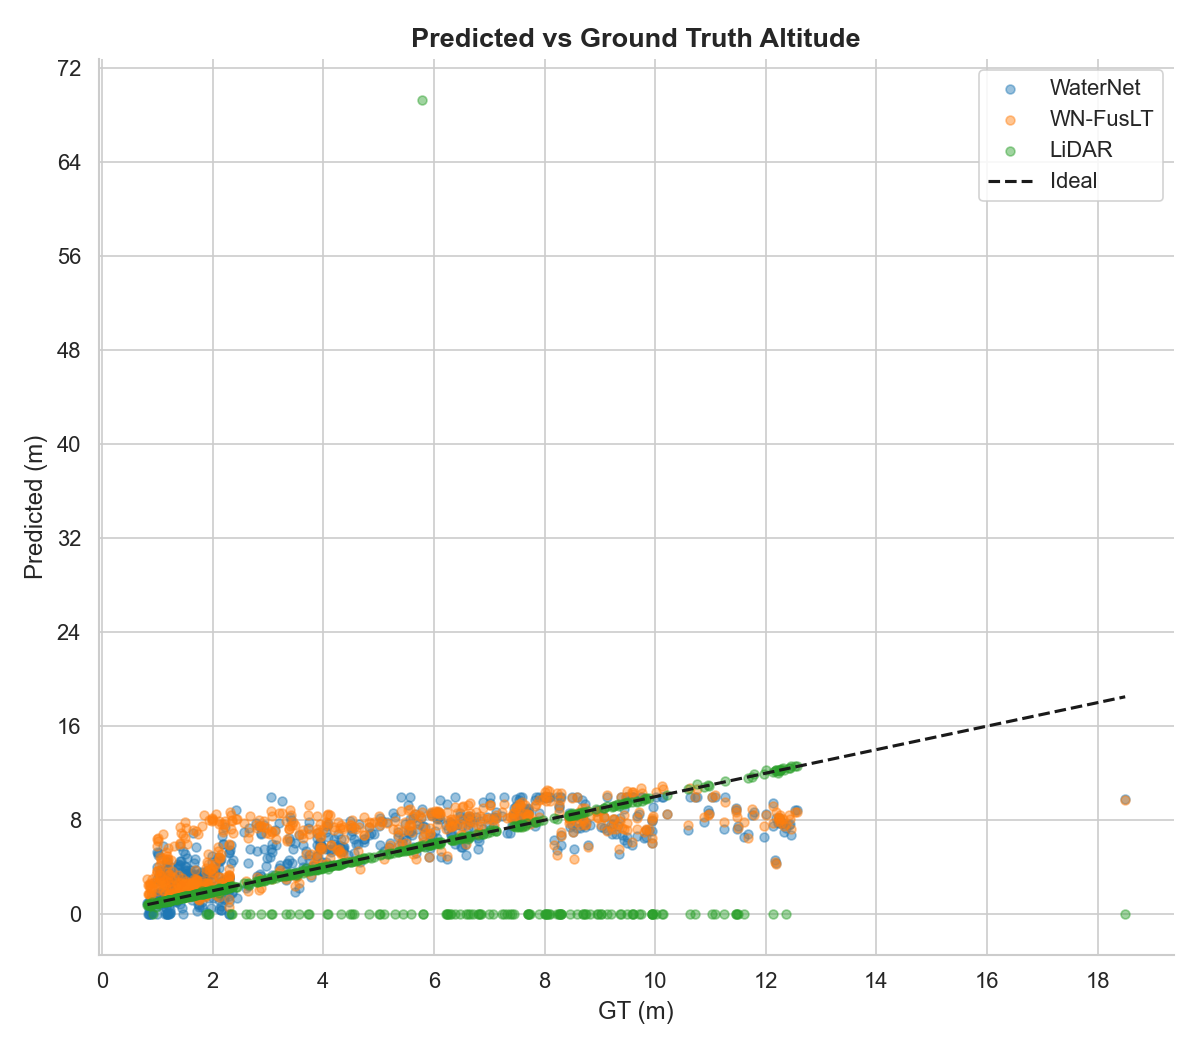
\includegraphics[width=14cm]{Images/waternet_benchmark_scatter.png}
    \caption{Predicted vs.\ ground-truth altitude for WaterNet, WaterNet-FusionLite, and LiDAR. The dashed line represents ideal predictions.}
    \label{fig:waternet_scatter}
\end{figure}

\subsubsection{LiDAR Sensor Analysis}
\label{subsec:lidar_analysis}

The LiDAR sensor was included in the evaluation as a reference for the conventional approach to altitude measurement. However, the results confirm the fundamental limitation described in the introduction: LiDAR is unreliable over water surfaces. Of the 4{,}100 frames, 857 (20.9\%) produced near-zero readings (below 0.1~m), indicating complete signal loss due to specular reflection or absorption at the water surface. At the other extreme, 6 frames produced readings exceeding 20~m, with a maximum of 77.1~m, likely caused by multipath reflections or sensor saturation. These failure modes explain the paradoxical combination of the lowest MAE (1.697~m, driven by the many frames where the sensor works correctly) and the highest RMSE (4.364~m, driven by the catastrophic outliers) among all evaluated methods. The negative $R^2$ value ($-0.567$) further confirms that the LiDAR performs worse than a constant mean predictor over this dataset.

This result validates the central motivation of the present work: over water surfaces, conventional ranging sensors can fail catastrophically and unpredictably, producing errors of an order of magnitude larger than the true altitude. A vision-based estimator, even with moderate average error, provides substantially more predictable and bounded behavior, which is a desirable property for flight control systems that rely on altitude estimates for safety-critical decisions.

% ──────────────────────────────────────────────
\subsection{Model Comparison}
\label{subsec:model_comparison}

Table~\ref{tab:model_comparison} provides a consolidated comparison of the four architectures across dimensions relevant to both research evaluation and practical deployment.

\begin{table}[htbp]
    \caption{Comprehensive comparison of the four evaluated architectures. Synthetic metrics refer to the test partition.}
    \begin{center}
        \small
        \begin{tabular}{|l|c|c|c|c|}
        \hline
        \textbf{Property}
            & \textbf{ResNet50}
            & \textbf{RN50-Fus}
            & \textbf{WaterNet}
            & \textbf{WN-FusLT} \\
        \hline
        \multicolumn{5}{|l|}{\textit{Architecture}} \\
        \hline
        Backbone
            & ResNet50
            & ResNet50
            & Custom (VGG)
            & Custom (VGG) \\
        Kernel size
            & $3\times3$/$1\times1$
            & $3\times3$/$1\times1$
            & $5\times5$
            & $3\times3$ \\
        Conv.\ blocks
            & 16 (residual)
            & 16 (residual)
            & 4
            & 3 \\
        Feature input
            & No
            & Yes (12-dim)
            & No
            & Yes (12-dim) \\
        Fusion strategy
            & ---
            & Yes
            & ---
            & Yes \\
        \hline
        \multicolumn{5}{|l|}{\textit{Size and complexity}} \\
        \hline
        Total parameters
            & 24.1\,M
            & 23.9\,M
            & 3.5\,M
            & 310\,K \\
        Trainable (Stage~1)
            & 558\,K
            & 286\,K
            & 3.5\,M
            & 310\,K \\
        Pretrained backbone
            & ImageNet
            & ImageNet
            & None
            & None \\
        \hline
        \multicolumn{5}{|l|}{\textit{Training behavior}} \\
        \hline
        Convergence speed
            & Slow ($\sim$50 ep.)
            & Moderate ($\sim$80 ep.)
            & Fast ($\sim$20 ep.)
            & Moderate ($\sim$35 ep.) \\
        Overfitting tendency
            & Moderate
            & Low
            & Low
            & Low \\
        \hline
        \multicolumn{5}{|l|}{\textit{Synthetic test performance}} \\
        \hline
        Error $\mu$ (cm)
            & $-1.7$
            & $+0.8$
            & $+18.7$
            & $-7.6$ \\
        Error $\sigma$ (cm)
            & 98.1
            & 44.3
            & 40.3
            & 41.7 \\
        \hline
        \multicolumn{5}{|l|}{\textit{Real-world performance}} \\
        \hline
        MAE (m)
            & 2.700
            & 2.824
            & \textbf{1.787}
            & 2.208 \\
        RMSE (m)
            & 3.591
            & 3.266
            & \textbf{2.337}
            & 2.859 \\
        Bias (m)
            & $-1.455$
            & \textbf{0.118}
            & 0.518
            & 1.192 \\
        $R^2$
            & $-0.061$
            & 0.122
            & \textbf{0.551}
            & 0.327 \\
        \hline
        \multicolumn{5}{|l|}{\textit{Deployment considerations}} \\
        \hline
        Edge suitability
            & Low
            & Low
            & Moderate
            & High \\
        Requires feature eng.
            & No
            & Yes
            & No
            & Yes \\
        \hline
        \end{tabular}
    \label{tab:model_comparison}
    \end{center}
\end{table}

\subsubsection{Effect of Transfer Learning vs.\ Domain-Specific Training}

A counterintuitive finding of this evaluation is that the custom WaterNet architecture, trained from scratch on synthetic water surface imagery, outperforms the ResNet50-based models that leverage ImageNet-pretrained weights. This result contrasts with the common assumption in computer vision that transfer learning from large-scale datasets universally improves performance, and deserves careful interpretation.

The ResNet50 backbone was pretrained on ImageNet, a dataset dominated by natural images of objects, animals, and scenes with rich semantic content and well-defined structural features. The features learned from such data --- edges, textures, shapes, and object parts --- are optimized for classification tasks where the goal is to distinguish between semantically different categories. In contrast, altitude estimation over water requires discriminating between images of the same visual category (water surface) based on subtle differences in texture scale, brightness distribution, and specular reflection density. These differences are encoded in low-level and mid-level features that may be overridden or compressed by the deep representations learned for classification.

The WaterNet architecture, with its four convolutional blocks of $5\times5$ kernels, is specifically designed to capture large receptive fields at moderate depth, which aligns well with the spatial scale of the altitude-dependent texture features. The $5\times5$ kernels in the early layers capture local wave patterns and brightness gradients more directly than the $3\times3$ kernels used throughout ResNet50, where equivalent receptive fields require stacking multiple layers and traversing residual connections.

\subsubsection{Effect of Feature Fusion}

The impact of the handcrafted feature vector is asymmetric across the two backbone families. For the ResNet50 family, fusion produces a dramatic improvement: it reduces the error standard deviation from 98.1 to 44.3~cm on the synthetic test set and shifts the real-world bias from $-1.455$ to $+0.118$~m. This improvement indicates that the handcrafted features provide altitude-correlated information that the frozen ResNet50 backbone fails to extract from the image alone, effectively compensating for the backbone's domain mismatch.

For the WaterNet family, fusion produces a more nuanced effect. The WaterNet-FusionLite model achieves a lower bias magnitude ($-7.6$ vs.\ $+18.7$~cm on synthetic; $+1.192$ vs.\ $+0.518$~m on real) but higher MAE and RMSE than the standalone WaterNet. This suggests that the handcrafted features help center the predictions but introduce additional variance, possibly because the lighter convolutional backbone (3 blocks, $3\times3$ kernels) produces less discriminative image embeddings that the fusion head cannot fully compensate for.